\documentclass[10pt,a4paper,english]{article}
\usepackage{geometry,metalogo,hyperref,babel,mdwlist,array,multicol}
\usepackage[default,osf]{sourcesans}
\usepackage[scaled=.95]{sourcecodepro}

\hypersetup{
    colorlinks,
    citecolor=blue,
    filecolor=blue,
    linkcolor=blue,
    urlcolor=blue
}
\newcommand*\file[1]{\href{run:#1.pdf}{#1}}

\title{\bfseries
	\Huge sourcesans\\
	\Large Adobe's Source Sans typeface for \LaTeX
}

\author{Silke Hofstra, \href{mailto:tex@slxh.nl}{tex@slxh.nl}}
\date{Documentation for sourcesans v3.0.\\ \today}

\begin{document}
\maketitle
\begin{multicols}{2}
This package provides the Source Sans font in an easy to use way. For \XeLaTeX\ and \LuaLaTeX\ users the original OpenType fonts from \href{https://github.com/adobe-fonts/source-sans}{GitHub} are used. The entire font family is included.

This package is also available on \href{https://gitlab.com/slxh/latex/sourcesans}{GitLab}.


\section{Options}
The package has the following options:
\begin{itemize*}
	\item \textbf{oldstyle, osf}:  use old style numbers.
	\item \textbf{lining, nf, lf}: use lining numbers.
	\item \textbf{tabular}:        use fixed-width numbers.
	\item \textbf{proportional}:   use normal numbers.
	\item \textbf{black}:          \texttt{\textbackslash bfseries} is black.
	\item \textbf{semibold}:       \texttt{\textbackslash bfseries} is semibold.
	\item \textbf{bold}:           \texttt{\textbackslash bfseries} is bold.
	\item \textbf{light}:          \texttt{\textbackslash mdseries} is light.
	\item \textbf{extralight}:     \texttt{\textbackslash mdseries} is extra light.
	\item \textbf{regular}:        \texttt{\textbackslash mdseries} is regular.
	\item \textbf{medium}:         \texttt{\textbackslash mdseries} is medium.
	\item \textbf{scale, scaled}:  Change the scaling with a factor. For example:  \texttt{scale=.5}
	\item \textbf{default}:        Source Sans is set as the default font family and as the sans serif family.
	\item \textbf{nosfdefault}:    Source Sans is not set as sans-serif family.
	\item \textbf{type1, t1}:      Override automatic detection and use the Type 1 fonts.
	\item \textbf{opentype, otf}:  Override automatic detection and use OpenType fonts.
\end{itemize*}
The following options are enabled by default: lining, tabular, bold and regular.

\section{Commands}
Commands for all weights are also provided for \XeLaTeX\ and \LuaLaTeX\ users.
\begin{itemize*}
	\item \texttt{\bfseries \textbackslash sourcesans}
		-- the regular and bold weights.
	\item \texttt{\bfseries \textbackslash sourcesansmedium}
		-- the medium and bold weights.
	\item \texttt{\bfseries \textbackslash sourcesanslight}
		-- the light and semibold weights.
	\item \texttt{\bfseries \textbackslash sourcesansextreme}
		-- the extra light and black weights.
\end{itemize*}

\section{Licence}
Adobe's Source Sans typeface is available under the \href{http://scripts.sil.org/OFL}{SIL Open Font License 1.1}.\\
All \LaTeX\ code is available under the \href{http://www.latex-project.org/lppl/}{\LaTeX\ project public license} v1.3 or later.

\section{Specimen}
Simple specimen can be found on page \pageref{sec:specimen}. Full specimen can be \href{http://adobe-fonts.github.io/source-sans-pro/}{acquired from Adobe}.

\section{OpenType}
The OpenType fonts have many features, including old style numerals (1 6 9),  ligatures (ff fi fl ft {\addfontfeature{Style=Alternate}fl}) and stylistic alternatives ({\addfontfeature{Style=Alternate} l a g I}).

\subsection{Features}
A complete list of available font features is available on page \pageref{sec:otfinfo}. More information on how to use font features can be found in the \href{http://mirror.ctan.org/macros/latex/contrib/fontspec/fontspec.pdf}{fontspec documentation}.

\subsection{Files}
\begin{itemize*}
	\item SourceSans3-ExtraLight.otf
	\item SourceSans3-ExtraLightIt.otf
	\item SourceSans3-Light.otf
	\item SourceSans3-LightIt.otf
	\item SourceSans3-Regular.otf
	\item SourceSans3-RegularIt.otf
	\item SourceSans3-Medium.otf
	\item SourceSans3-MediumIt.otf
	\item SourceSans3-Semibold.otf
	\item SourceSans3-SemiboldIt.otf
	\item SourceSans3-Bold.otf
	\item SourceSans3-BoldIt.otf
	\item SourceSans3-Black.otf
	\item SourceSans3-BlackIt.otf
\end{itemize*}

\section{Type1}
The following Type1 font families are included:
\begin{itemize*}
	\item SourceSansThree-LF
	\item SourceSansThree-TLF
	\item SourceSansThree-OsF
	\item SourceSansThree-TOsF
\end{itemize*}

With series ‘extralight’ (‘el’), ‘light’ (‘l’), ‘regular’ (‘m’), ‘medium’, ‘semibold’ (‘sb’), ‘bold’ (‘b’), ‘black’ (‘eb’) and shapes ‘n’, ‘i’ and ‘sc’.

\section{Version history}
\subsection*{3.1}
\begin{itemize*}
    \item Use standard names for font series.
\end{itemize*}

\subsection*{3.0}
\begin{itemize*}
	\item Update fonts to version 3.052
	\item Rename package to \texttt{sourcesans}
	\item Add medium weight
\end{itemize*}

\subsection*{2.8}
\begin{itemize*}
	\item Updated fonts to version 3.006.
\end{itemize*}

\subsection*{2.7}
\begin{itemize*}
	\item Updated fonts to Roman 2.045 and Italic 1.095.
	\item Tabular numbers are now default in order to match the original font behaviour.
\end{itemize*}

\subsection*{2.6}
\begin{itemize*}
	\item Updated fonts to Roman 2.020 and Italic 1.075.
	\item Modified the \texttt{\textbackslash liningnums} to accomodate for the missing \texttt{lnum} feature.
	\item Experimental support for the LGR (Greek) encoding.
\end{itemize*}

\subsection*{2.5}
\begin{itemize*}
	\item Updated fonts to 2.010
\end{itemize*}

\subsection*{2.4}
\begin{itemize*}
	\item Fixed errors in weight implementation.
	\item Updated fonts to 1.065
\end{itemize*}

\subsection*{2.3}
\begin{itemize*}
	\item Weights are now handled with the \href{http://www.ctan.org/pkg/mweights}{mweights} package.
\end{itemize*}

\subsection*{2.2}
\begin{itemize*}
	\item Updated fonts to 1.050
	\item Added \texttt{nosfdefault} option.
\end{itemize*}

\subsection*{2.1}
\begin{itemize*}
	\item Updated fonts to 1.040
\end{itemize*}

\subsection*{2.0}
\begin{itemize*}
	\item Merged all \texttt{.sty} files into \texttt{sourcesans.sty}.
	\item \texttt{default} option now sets the default font family to \texttt{Source Sans}, not \texttt{\textbackslash sfdefault}.
	\item \texttt{type1}, \texttt{t1}, \texttt{opentype} and \texttt{otf} option added to override automatic detection.
	\item Added \texttt{OT1} to \texttt{fontspec} options.
\end{itemize*}

\subsection*{1.02}
\begin{itemize*}
	\item Changed the order of \texttt{T1} and \texttt{LY1}.
	\item Changed \texttt{lining}/\texttt{nf} behaviour.
	\item Redefined \texttt{\textbackslash oldstylenums}.
\end{itemize*}

\section{Known issues}

Issues can be reported \href{https://gitlab.com/slxh/latex/sourcesans/issues}{on GitLab} and \href{https://github.com/silkeh/latex-sourcesanspro/issues}{GitHub}.

\newpage
\end{multicols}

\section{Specimen}
\label{sec:specimen}
\subsection{OpenType}
\begin{figure}[ht]
	\centering
	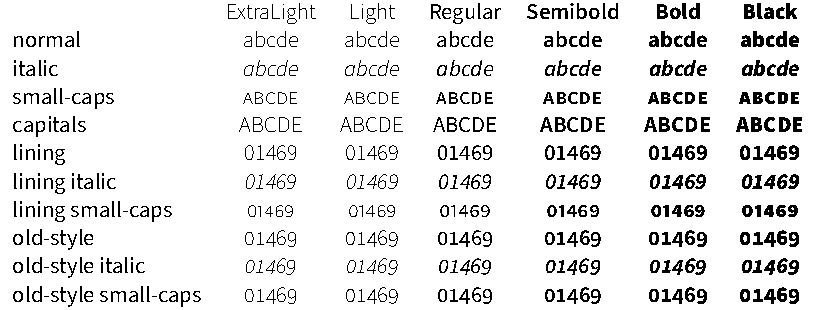
\includegraphics{sourcesans-otf-specimen}
\end{figure}
This table can also be found in \file{sourcesans-otf-specimen}.

\subsection{Type1}
\begin{figure}[ht]
	\centering
	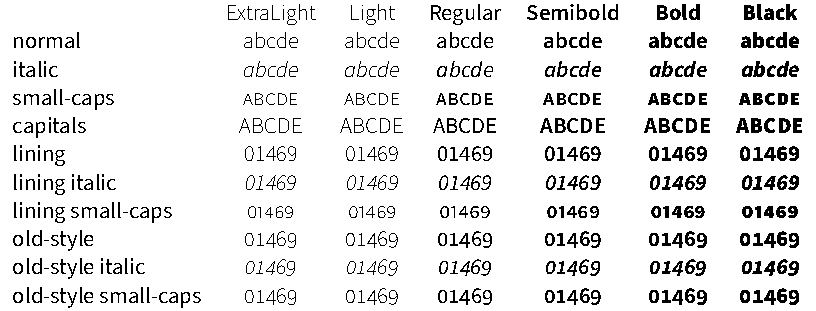
\includegraphics{sourcesans-type1-specimen}
\end{figure}
This table can also be found in \file{sourcesans-type1-specimen}.

\newpage
\section{Opentype features}
\label{sec:otfinfo}

\begin{figure}[ht]
	\centering
	\begin{tabular}{>{\ttfamily}l l}
        aalt & Access All Alternates \\
        c2sc & Small Capitals From Capitals \\
        case & Case-Sensitive Forms \\
        ccmp & Glyph Composition/Decomposition \\
        cv01 & Character Variants 1 \\
        cv02 & Character Variants 2 \\
        cv03 & Character Variants 3 \\
        cv04 & Character Variants 4 \\
        cv05 & Character Variants 5 \\
        cv06 & Character Variants 6 \\
        cv07 & Character Variants 7 \\
        cv08 & Character Variants 8 \\
        cv09 & Character Variants 9 \\
        cv10 & Character Variants 10 \\
        cv11 & Character Variants 11 \\
        cv12 & Character Variants 12 \\
        cv13 & Character Variants 13 \\
        cv14 & Character Variants 14 \\
        cv15 & Character Variants 15 \\
        cv16 & Character Variants 16 \\
        cv17 & Character Variants 17 \\
        cv18 & Character Variants 18 \\
        cv19 & Character Variants 19 \\
        dlig & Discretionary Ligatures \\
        dnom & Denominators \\
        frac & Fractions \\
        hlig & Historical Ligatures \\
        kern & Kerning \\
        liga & Standard Ligatures \\
        locl & Localized Forms \\
        mark & Mark Positioning \\
        mkmk & Mark to Mark Positioning \\
        numr & Numerators \\
        onum & Oldstyle Figures \\
        ordn & Ordinals \\
        pnum & Proportional Figures \\
        salt & Stylistic Alternates \\
        sinf & Scientific Inferiors \\
        size & Optical Size \\
        smcp & Small Capitals \\
        ss01 & Stylistic Set 1 - alternate l \\
        ss02 & Stylistic Set 2 - alternate a \\
        ss03 & Stylistic Set 3 - alternate g \\
        ss04 & Stylistic Set 4 - alternate I \\
        ss05 & Stylistic Set 5 - \\
        ss06 & Stylistic Set 6 \\
        ss07 & Stylistic Set 7 \\
        ss08 & Stylistic Set 8 \\
        ss09 & Stylistic Set 9 \\
        ss10 & Stylistic Set 10 \\
        subs & Subscript \\
        sups & Superscript \\
        titl & Titling \\
        zero & Slashed Zero \\
	\end{tabular}
\end{figure}
\textit{(list generated with otfinfo)}

\end{document}
